% Compile with: pdflatex intro_meme.tex
% "Galaxy brain" meme for the project intro.
% Four panels of escalating sophistication, ending in the actual approach.

\documentclass[11pt]{article}
\usepackage[a4paper, margin=15mm]{geometry}
\usepackage{tikz}
\usepackage{amsmath}
\usetikzlibrary{shapes.symbols, shapes.geometric, decorations.pathmorphing,
                shadings, calc}
\pagestyle{empty}

\definecolor{brainA}{RGB}{248,200,210}
\definecolor{brainB}{RGB}{240,160,180}
\definecolor{brainC}{RGB}{180,140,210}
\definecolor{brainD}{RGB}{160,190,230}

\newcommand{\brain}[3]{%
  % #1 = center coords, #2 = scale, #3 = base color name
  \begin{scope}[shift={#1}, scale=#2]
    \draw[fill=#3, draw=black!50, line width=0.4pt,
          decorate, decoration={random steps, segment length=2pt, amplitude=0.4pt}]
      (0,0) circle (0.9);
    \draw[black!40, line width=0.4pt] (0,0.85) .. controls (-0.05,0.2) and (0.05,-0.2) .. (0,-0.85);
    \foreach \a in {30, 75, 120, 200, 240, 300, 340}{
      \draw[black!40, line width=0.3pt, decorate,
            decoration={coil, aspect=0, segment length=2pt, amplitude=0.7pt}]
        (\a:0.55) -- (\a:0.85);
    }
  \end{scope}
}

\newcommand{\sparkles}[2]{%
  % #1 = center, #2 = radius
  \foreach \a/\r in {15/#2, 70/{#2*0.85}, 130/{#2*1.05}, 200/{#2*0.9},
                     260/{#2*1.0}, 320/{#2*0.95}}{
    \node[star, star points=5, star point ratio=2.4, fill=yellow!85!orange,
          draw=orange!80!black, line width=0.2pt,
          inner sep=0pt, minimum size=2.4pt] at ($#1+(\a:\r)$) {};
  }
}

\newcommand{\galaxysparkles}[2]{%
  \foreach \a/\r/\s in {10/#2/3.5, 55/{#2*0.9}/2.8, 100/{#2*1.1}/4.0,
                        150/{#2*0.95}/2.6, 190/{#2*1.05}/3.2,
                        235/{#2*0.85}/4.2, 280/{#2*1.0}/2.8,
                        325/{#2*1.08}/3.6}{
    \node[star, star points=5, star point ratio=2.4,
          fill=yellow!85!orange, draw=orange!80!black, line width=0.2pt,
          inner sep=0pt, minimum size=\s pt] at ($#1+(\a:\r)$) {};
  }
  % little dots for distant stars
  \foreach \a/\r in {25/{#2*1.2}, 80/{#2*1.25}, 165/{#2*1.15},
                     215/{#2*1.3}, 290/{#2*1.2}, 340/{#2*1.18}}{
    \fill[white] ($#1+(\a:\r)$) circle (0.5pt);
  }
}

\begin{document}

\begin{center}
{\Large\bfseries Detecting AI-generated images: a journey}\\[2mm]
{\small (ADAIS / wave\_1)}\\[6mm]
\end{center}

\begin{center}
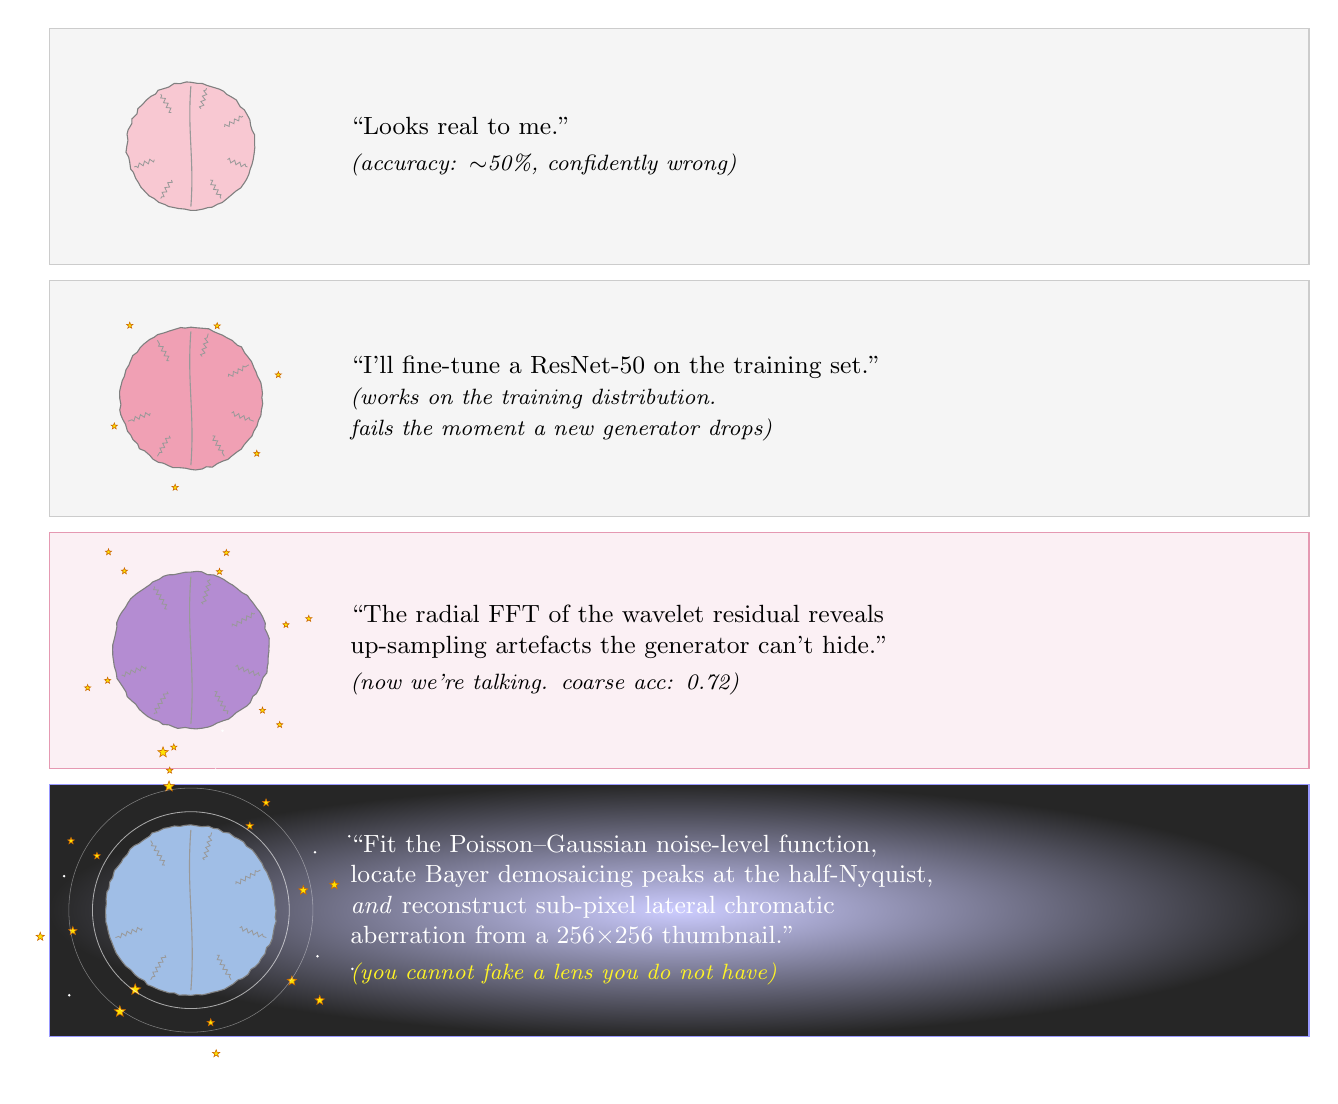
\begin{tikzpicture}[every node/.style={font=\small}]

% --- panel 1: just look ----------------------------------------------------
\fill[gray!8] (0,0) rectangle (16, 3);
\draw[gray!40] (0,0) rectangle (16, 3);
\brain{(1.8,1.5)}{0.9}{brainA}
\node[align=left, anchor=west, text width=110mm] at (3.7, 1.5)
  {``Looks real to me.''\\[2pt]
   \footnotesize\itshape (accuracy: $\sim$50\%, confidently wrong)};

% --- panel 2: throw a CNN at it -------------------------------------------
\fill[gray!8] (0,-3.2) rectangle (16, -0.2);
\draw[gray!40] (0,-3.2) rectangle (16, -0.2);
\brain{(1.8,-1.7)}{1.0}{brainB}
\sparkles{(1.8,-1.7)}{1.15}
\node[align=left, anchor=west, text width=110mm] at (3.7, -1.7)
  {``I'll fine-tune a ResNet-50 on the training set.''\\[2pt]
   \footnotesize\itshape (works on the training distribution.\\
                          fails the moment a new generator drops)};

% --- panel 3: frequency domain --------------------------------------------
\fill[purple!6] (0,-6.4) rectangle (16, -3.4);
\draw[purple!40] (0,-6.4) rectangle (16, -3.4);
\brain{(1.8,-4.9)}{1.1}{brainC}
\sparkles{(1.8,-4.9)}{1.25}
\sparkles{(1.8,-4.9)}{1.55}
\node[align=left, anchor=west, text width=110mm] at (3.7, -4.9)
  {``The radial FFT of the wavelet residual reveals\\
    up-sampling artefacts the generator can't hide.''\\[2pt]
   \footnotesize\itshape (now we're talking. coarse acc: 0.72)};

% --- panel 4: galaxy brain -------------------------------------------------
\shade[inner color=blue!20, outer color=black!85]
   (0,-9.8) rectangle (16, -6.6);
\draw[blue!40] (0,-9.8) rectangle (16, -6.6);
\brain{(1.8,-8.2)}{1.2}{brainD}
\galaxysparkles{(1.8,-8.2)}{1.45}
\galaxysparkles{(1.8,-8.2)}{1.85}
% halo
\draw[white!80, line width=0.3pt, opacity=0.6] (1.8,-8.2) circle (1.25);
\draw[white!80, line width=0.2pt, opacity=0.4] (1.8,-8.2) circle (1.55);

\node[align=left, anchor=west, text width=110mm, text=white] at (3.7, -8.2)
  {``Fit the Poisson--Gaussian noise-level function,\\
    locate Bayer demosaicing peaks at the half-Nyquist,\\
    \emph{and} reconstruct sub-pixel lateral chromatic\\
    aberration from a $256{\times}256$ thumbnail.''\\[2pt]
   \footnotesize\itshape\color{yellow!85!white}
    (you cannot fake a lens you do not have)};

\end{tikzpicture}
\end{center}

\vspace{4mm}
\begin{center}
\itshape\small
The classifier doesn't ask ``does this look fake?''\\
It asks ``does this look like it came out of a \emph{camera}?''
\end{center}

\end{document}
